\documentclass[../main.tex]{subfiles}
\begin{document}

\chapter{Lecture 14 - 28-04-2020}

\section{Linear Regression}
Yesterday we look at the problem of emprical risk  minismisation for a linear classifier. 0-1 loss is not good: discontinuous jumping from 0 to 1 and it's dififcult to optimise. Maybe with linear regression we are luckier.
\\
Our data point are the form $(x,y) \ x \in \barra{R}^d \ $ regression, $(\hat{y}-y)^2$ square loss. 
\\
We are able to pick a much nicer function and we can optimise it in a easier way.
\\
\subsection{The problem of linear regression}
Instead of picking -1 or 1 we just leave it as it is. 
$$h(c) = w^T \ x \qquad w \in \barra{R}^d \qquad x = (x_1, ..., x_d, 1) $$
\\
$$
\hat{w} = arg \min_{w \in \barra{R}^d} \frac{1}{m} \sum_{t=1}^{m} (w^T \ x_t- y_t ) ^2 \qquad \textit{ERM for } \ (x_1,y_1) ... (x_m, y_m)
$$
How to compute the minimum? \\
We use the vector v of linear prediction\\
$v = (w^T x_1, .., w^T x_m )$
\\
and a vector of real valued labels\\
$y = (y_1, ..., y_m) $ where $v, y \in \barra{R}^m$
\\
$$
\sum_{t=1}^{m} (w^T x_t - y_t ) ^2  \ = \ \| v - y\|^2 
$$
S is a matrix.
$$
s^T = \left[ x_1, ... , x_m \right] \quad d \times m
\qquad
v = s w = 
\begin{bmatrix}
x^t_1 \\ ...\\  x^T_m
\end{bmatrix}
\begin{bmatrix}
\\
w
\\\\
\end{bmatrix}
$$
So:
$$
\ \| v - y\|^2  = \| sw - y\|^2
$$
$$
\hat{w} = arg \min_{w \in \barra{R}^d} \| sw - y \| ^2 \qquad \textbf{where $sw$ is the design matrix}
$$
$$
F (w) = \| sw - y \|^2 \qquad \bred{is convex}
$$
$$
\nabla F(w) = \not2 s^T \left( sw - y \right) = 0 \qquad s^T\ s w = s^T y
$$
where $s^T$ is $d \times m$ and $s$ is $m \times d$ and $ d \neq m$
\\
If $s^T \ s$ invertible (non singular)
$ \hat{w} = (s^T \ s)^{-1} \ s^T \ y $\\
And this is called \bred{ Least square solutions (OLS)}
\\\\
We can check $s^T\ s$ is non-singular if $x_1, ... , x_m$ span $\barra{R}^d$
\\\\
$s^T \cdot s$ may not be always invertible. Also Linear regression is high bias solution. ERM may underfit since linear predictor introduce big bias.
\\
$ \hat{w} = ( s^T \cdot s)^{-1} \cdot s^T \cdot y $ is very instable: can change a lot when the the dataset is perturbed.
\\
This fact is called \bred{instability} : variance error
\\
It is a good model to see what happens and then try more sofisticated model. 
\\
Whenever $\hat{w}$ is invertible we have to prove the instability. But there is a easy fix!
\\\\
\subsection{Ridge regression}
We want to stabilised our solution. If $s^T \cdot s$ non-singular is a problem.
\\\\
We are gonna change and say something like this:
$$
\hat{w} = arg \min_w \| s \cdot w - y \|^2 \quad \rightsquigarrow \hat{w}_\alpha = arg \min_w \left(\| s \, w - y \|^2 + \alpha \cdot \| w \|^2 \right)
$$
where $\alpha$ is the \textbf{regularisation term.}
\\\\
$
\hat{w}_\alpha \rightarrow \hat{w} 
$ for $\alpha \rightarrow 0$
\\
$
\hat{w}_\alpha \rightarrow (0,..., 0) 
$ for $\alpha \rightarrow \infty$\\
\begin{figure}[h]
    \centering
    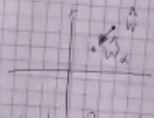
\includegraphics[width=0.3\linewidth]{../img/lez14-img1.JPG}
    \caption{}
    %\label{fig:}
\end{figure}\\
\\
$\hat{w}_\alpha$ has more bias than $\hat{w}$, but also less variance
\\
$$\nabla \left( \| s \, w - y \|^2 + \alpha \, \| w \|^2 \right) \ = \ 2 \, \left( s^T \, s \, w - s^T \, y \right) + 2 \, \alpha \, w = 0$$
$$
\left(s^T \, s + \alpha \, I \right) \, w = s^T \, y
$$
$$
(d \times m) \, (m \times d) \ (d \times d) \ (d \times m) \qquad (d \times m) \ (m \times 1)
$$
where I is the identity
\\
$$
\hat{w}_\alpha = \left( s^T \, s + \alpha \, I \right)^{-1} \, s^T \, y
$$
where $y_1,..., y_\alpha$ are eigen-values of $s^T \, s$
\\
$ y_1,..., y_\alpha + \alpha > 0 $ eigenvalues of $s^T \, s+ \alpha I$
\\In this way we make it positive and semidefinite.\\
We can always compute the inverse and it is a more stable solution and stable means \bred{do not overfit}.

\section{Percetron}
Now we want to talk about algorithms. \\
Data here are processed in a sequential fashion one by one.\\
Each datapoint is processed in costant time $ \Theta \left( d \right)$\\
(check $y_t \, w^T \leq 0$ and in case $ w \leftarrow w + y_t \, x_t$) 
and the linear model can be stored in $\Theta (d)$ space.
\\
Sequential processing scales well with the number of datapoints.
\\ But also is good at dealing with scenarios where new data are generated at all times.
\\ Several scenario like:
\begin{itemize}
\item Sensor data
\item Finantial data
\item Logs of user
\end{itemize}
So sequential learning is good when we have lot of data and scenario in which data comes in fits like sensor. 
\\ We call it \bred{Online learning}
\\
\subsection{Online Learning }
It is a learning protocol and we can think of it like Batch learning.
We have a class $H$ of predictors and a loss function $\ell$ and we have and algorith that outputs an initial default predictor $h_1 \in H$.
\\\\
For $t = 1,2 ...$\\
1) Next example $(x_t, y_t)$ is observed \\
2) The loss $\ell ( h_t(x_t), y_t)$ is observed \qquad $(y_t \, w^T \, x_t \leq 0 )$
\\
3) The algorithm updates $h_t$ generating $h_{t+1}$ \qquad $(w \leftarrow w + y_t \, x_t)$
\\\\
The algorithm generates $s$ sequence $h_1, h_2, ...$ of models\\
It could be that $h_{t+1} = h_t$ occasionally 
\\
The update $h_t \rightarrow h_{t+1}$ is \textbf{local} (it only uses $h_t$ and $(x_t, y_t)$)
\\
This is a batch example in which take the training set and generate a new example.
$$
(x_1,y_1) \rightarrow A \rightarrow h_2
$$
$$
(x_1,y_1) (x_2,y_2) \rightarrow A \rightarrow h_3
$$
But if I have a non-learning algorithm i can look at the updates: 
\begin{figure}[h]
    \centering
    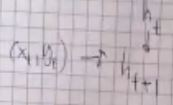
\includegraphics[width=0.3\linewidth]{../img/lez14-img2.JPG}
    \caption{}
    %\label{fig:}
\end{figure}\\
This is a most efficient way and can be done in a costant time.
The batch learning usually have single predictor while the online learning uses a sequence of predictors.
\\\\
How do I evaluate an online learning algorithm A?
I cannot use a single model, instead we use a method called \bred{Sequential Risk}. \\
Suppose that I have $h_1, h_2 ...$ on some data sequence.
\\
$$
\frac{1}{m} \ \sum_{t=1}^{T} \ell(h_t(x), y_t) \qquad \textit{as a function of T}
$$
The loss on the next incoming example. 
\newpage
 I would like something like this: 
\begin{figure}[h]
    \centering
    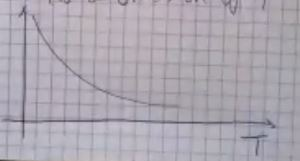
\includegraphics[width=0.3\linewidth]{../img/lez14-img3.JPG}
    \caption{}
    %\label{fig:}
\end{figure}\\\\
We need to fix the sequence of data: I absorb the example into the loss of the predictor.
$$
\ell(h_t(x), y_t) \longrightarrow \ell_t(h_t)
$$
I can write the sequential risk of the algorithm:
$$
\frac{1}{m} \sum_{t=1}^{T} \ell_t(h_t) - \min_{h \in H} \frac{1}{m} \sum_{t=1}^{T} \ell_t(h) 
$$
So the sequencial risk of the algorithm - the sequential risk of best predictor in $H$ (up to $T$).
\\
\bred{This is a sequential similar of variance error.} $\longrightarrow$ is called \textbf{Regret}.
\\

$$
h^*_T = arg \min_{h \in H} \frac{1}{T} \sum_{t} \ell_t(h) \qquad \frac{1}{T} \ell_t(h_t) - \frac{1}{T} \sum_t \ell_t(h_T^*)
$$
\newpage
\subsection{Online Gradiant Descent (OGD)}
It is an example of learning algorithm. \\
In optimisation we have one dimension and we want to minimise the function i can compute the gradiant in every point. \\
We start from a point and get the derivative: as I get the derivative I can see if is decreasing or increasing.\\
\begin{figure}[h]
    \centering
    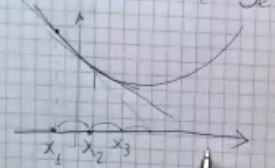
\includegraphics[width=0.3\linewidth]{../img/lez14-img4.JPG}
    \caption{}
    %\label{fig:}
\end{figure}\\

$$
f \quad convex \qquad \min_x f(x) \qquad f \ \barra{R}^d \rightarrow \barra{R}
$$
$$
x_{t+1} = x_t + \eta \nabla f(x_t)  \qquad \eta > 0
$$
$$
w_{t+1} =  w_t + \eta \, \nabla \ell_t(w_t)
$$
where $\eta$ is the learning rate.
$$
h(x) = w^T \, x \qquad \ell_t(w) = \ell( w^T \, x_t, y_t) \qquad \textit{for istance } \ \ell(w^T \, x_t, y_t) = (w^T \, x_t - y_t)^2
$$
Assumption $\ell_t$ is convex (to do optimisation easily) and differentiable (to compute the gradiant)
\end{document}